\documentclass[11pt]{article}

\usepackage{graphicx,amsmath,amssymb,amsfonts}
\usepackage[margin=1in]{geometry}
\usepackage{hyperref}
\usepackage{natbib}
\usepackage{color}

\renewcommand{\bottomfraction}{1.}
\renewcommand{\topfraction}{1.}
\renewcommand{\textfraction}{0}
\renewcommand{\floatpagefraction}{1.}

\graphicspath{{../correlation_analysis/figures/}}

% definition of \customlabel, which is used to label supplementary figures and tables
\makeatletter
\newcommand{\customlabel}[2]{%
\protected@write \@auxout {}{\string \newlabel {#1}{{#2}{\thepage}{}{}{}}}}
\makeatother

\customlabel{fig:cor_entropy_PC_screen_CSrmsf}{S1}
\customlabel{fig:cor_omega_PC_screen}{S2}
\customlabel{fig:cor_omega_PC_screen_CSrmsf}{S3}

\begin{document}

\noindent
\textbf{\large Supporting Figures for:\\Predicting evolutionary site variability from structure in viral proteins:\\buriedness, packing, flexibility, and design}

\noindent A. Shahmoradi, D. K. Sydykova, S. J. Spielman, E. L. Jackson, E. T. Dawson, A. G. Meyer,\\ C. O. Wilke
\bigskip

\centerline{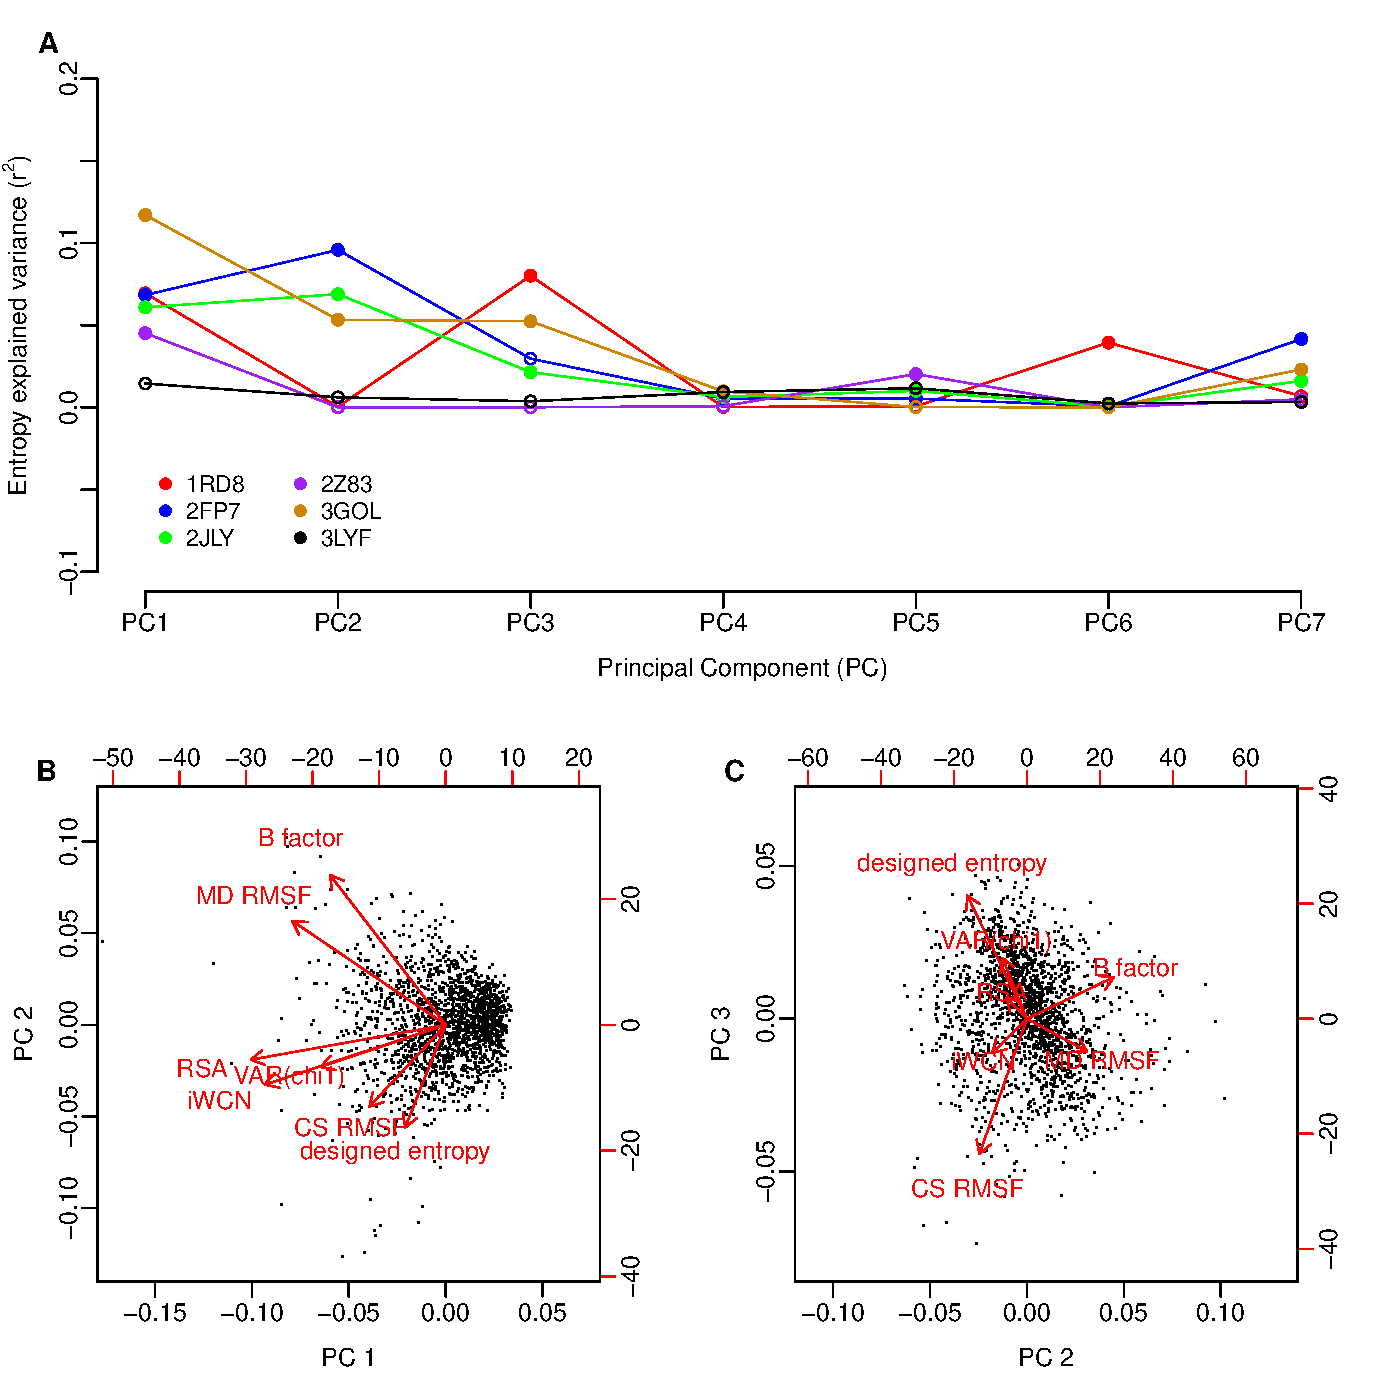
\includegraphics[width=6in]{PC_screen_entropy_CSrmsf.pdf}}
\noindent \textbf{Fig. S1} Principal Component (PC) Regression of sequence entropy against the structural variables, including CS RMSF. {\bf (A)} Variance in entropy explained by each principal component. For most proteins, PC1 and either PC2 or PC3 show the strongest correlations with sequence entropy. Significant correlations ($P<0.05$) are shown as filled symbols, and insignificant correlations ($P\geq0.05$) are shown as open symbols. {\bf (B)} and {\bf (C)} Composition of the three leading components. Red arrows represent the loadings of each of the structural variables on the principal components; black dots represent the amino acid sites in the PC coordinate system.
\customlabel{fig:cor_entropy_PC_screen_CSrmsf}{S1}


\newpage
\centerline{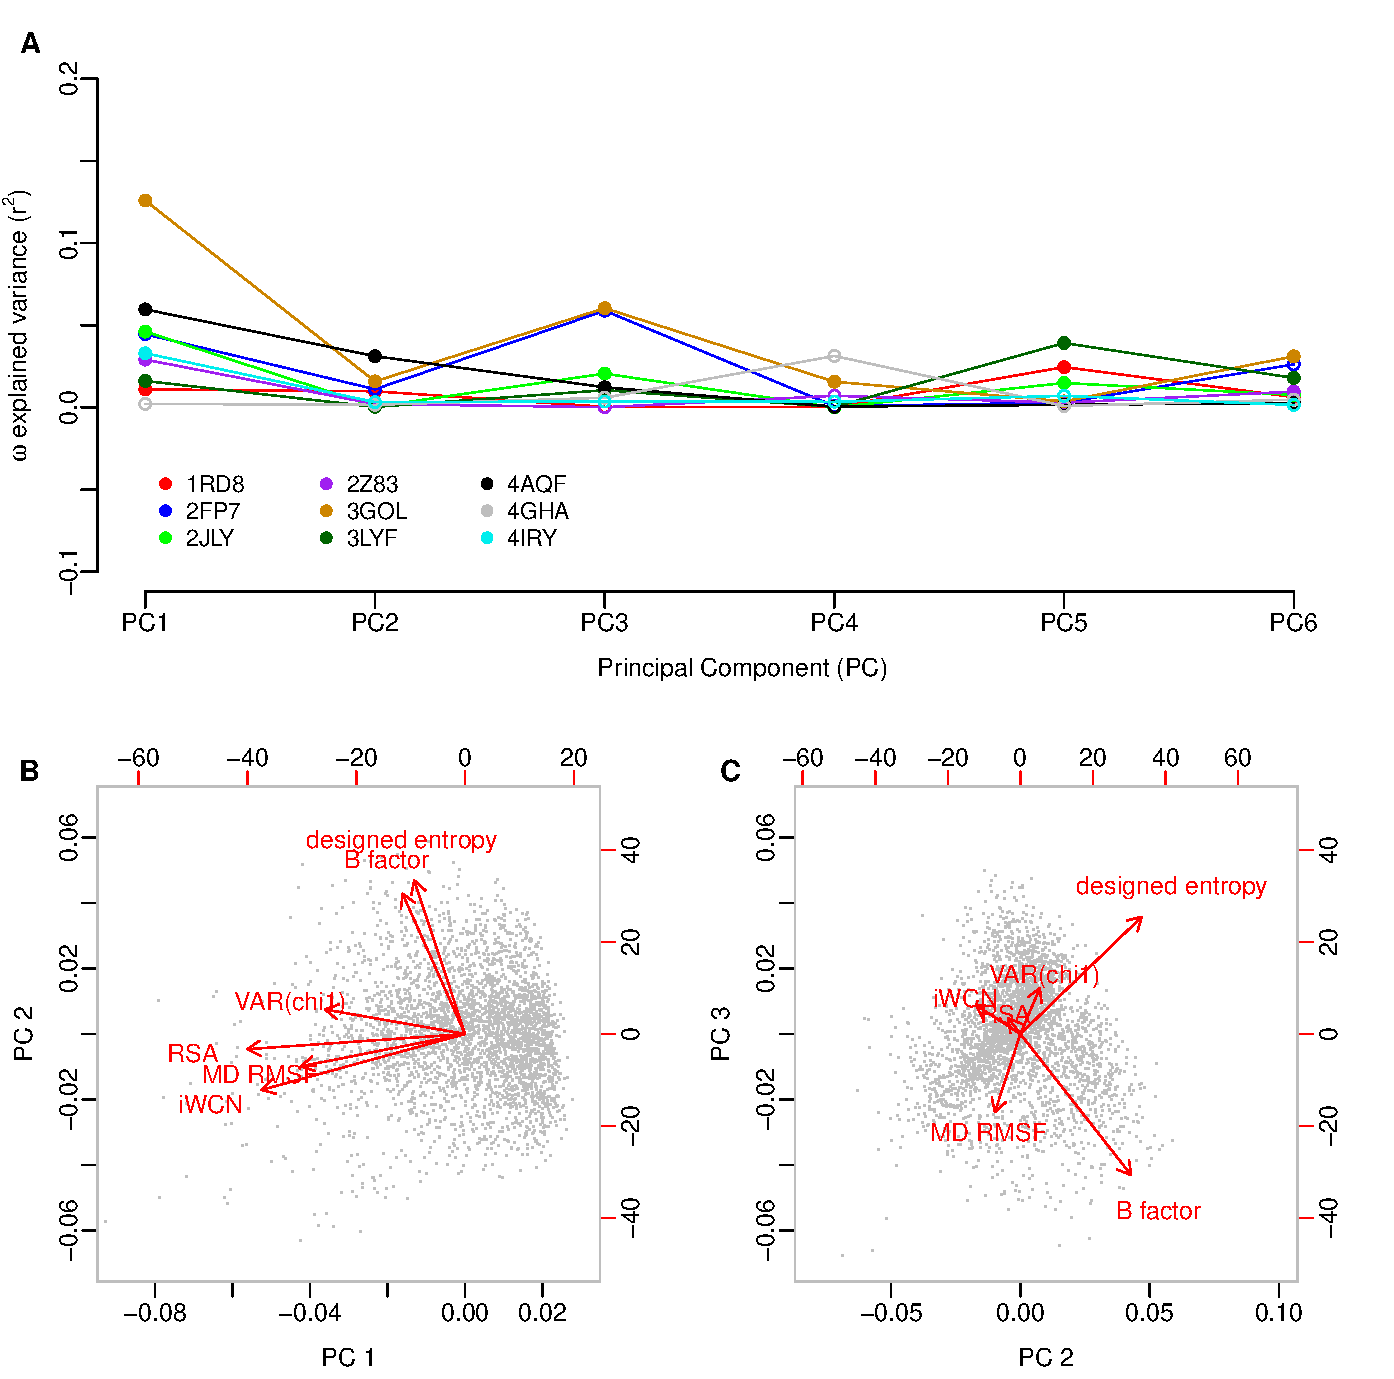
\includegraphics[width=6in]{PC_screen_omega.pdf}}
\noindent \textbf{Fig. S2} Principal Component (PC) Regression of $\omega$ against the structural variables. {\bf (A)} Variance in $\omega$ explained by each principal component. For most proteins, PC1 and PC3 show the strongest correlations with $\omega$. Significant correlations ($P<0.05$) are shown as filled symbols, and insignificant correlations ($P\geq0.05$) are shown as open symbols. {\bf (B)} and {\bf (C)} Composition of the three leading components. Red arrows represent the loadings of each of the structural variables on the principal components; black dots represent the amino acid sites in the PC coordinate system. Note that parts B and C are identical to those shown in Figure~6.%~\ref{fig:cor_entropy_PC_screen}.
\customlabel{fig:cor_omega_PC_screen}{S2}


\newpage
\centerline{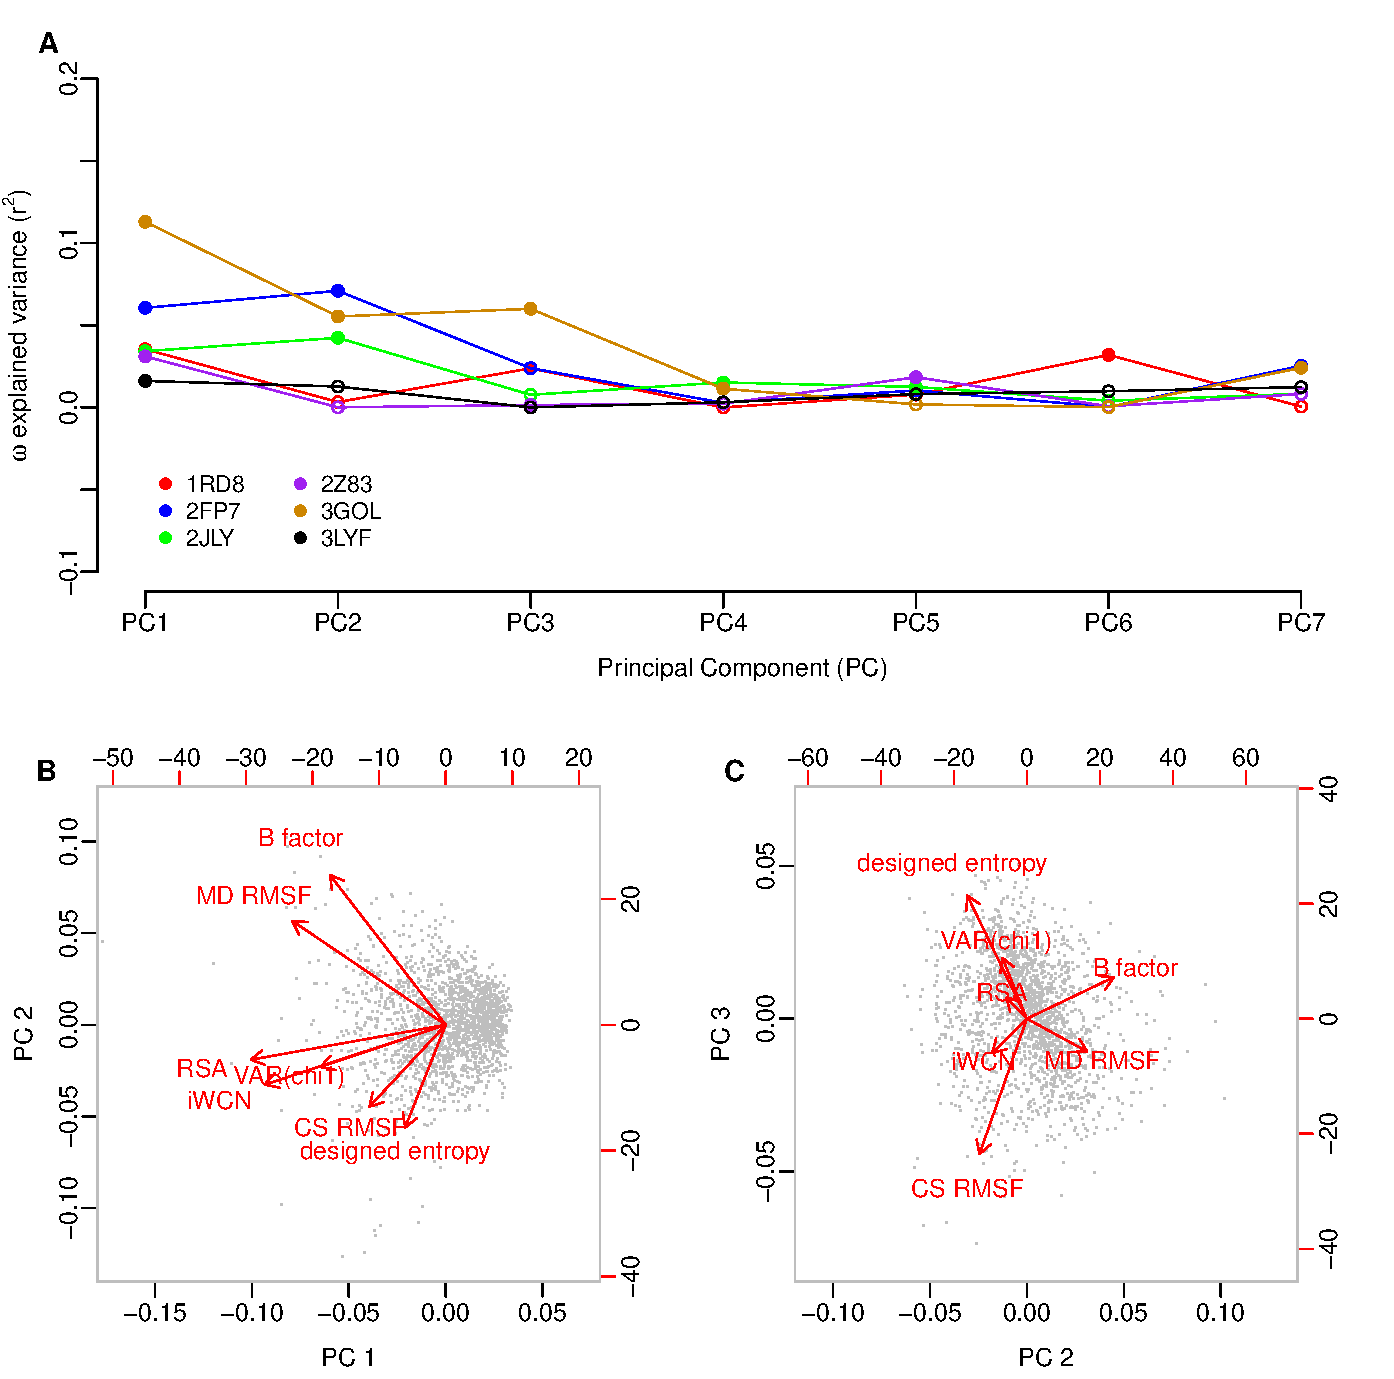
\includegraphics[width=6in]{PC_screen_omega_CSrmsf.pdf}}
\noindent \textbf{Fig. S3} Principal Component (PC) Regression of $\omega$ against the structural variables, including CS RMSF. {\bf (A)} Variance in $\omega$ explained by each principal component. For most proteins, PC1 and either PC2 or PC3 show the strongest correlations with $\omega$. Significant correlations ($P<0.05$) are shown as filled symbols, and insignificant correlations ($P\geq0.05$) are shown as open symbols. {\bf (B)} and {\bf (C)} Composition of the three leading components. Red arrows represent the loadings of each of the structural variables on the principal components; black dots represent the amino acid sites in the PC coordinate system. Note that parts B and C are identical to those shown in Figure~\ref{fig:cor_entropy_PC_screen_CSrmsf}.
\customlabel{fig:cor_omega_PC_screen_CSrmsf}{S3}

\end{document}
